\section{Hardware dell'adapter board}
L'hardware utilizzato per condurre lo studio oggetto di questa tesi consiste in due piattaforme indossabili per effettuare misure fotopletismografiche. Ciascuna piattaforma si compone di una Adapter Board e un microcontrollore. L'Adapter Board consiste in una PCB sulla quale sono montati il modulo PPG, un accelerometro ed un eventuale LDO per l'alimentazione dei componenti. Il microcontrollore viene utilizzato per l'acquisizione dei dati dai sensori e per il loro controllo. In particolare è stato utilizzata la board STM32F4DISCOVERY, prodotta da STMicroelectronics, in entrambi i casi.
La due piattaforme progettate si differenziano per l'Adapter Board, dal momento che sono stati utilizzati due differenti moduli PPG: il MAXM86161 e il MAX86916. Entrambi i sensori sono prodotti da Maxim Integrated.
\subsection{Adapter Board: MAXM86161}
\begin{figure}[h]
	\centering
	\includegraphics[width=0.8\linewidth]{ImageFiles/Hardware/diagramma_blocchi_MAXM}
	\caption{Diagramma a blocchi della piattaforma con sensore MAXM86161.}
	\label{fig:diagramma_blocchi_MAXM}
\end{figure} \todo{attenzione al accelerometro e al microcontrollore..  Metterei il nome con Discovery fuori dal riquadro arancione scuro (essendo la board) e dentro il nome del micor.... quasi quasi mettere l'immagine con sensore PPG generico sopra nell'introduzione così poi da lasciare qui e nel capitolo successivo le immagini del manufacturing (o layout ) delle board }
L'Adapter Board è la scheda che monta il sensore PPG utilizzato per fare le acquisizioni che, vengono fatte con il microcontrollore STM32F4DISCOVERY.\todo{stessi commenti sui nomi .. questa cosa in generale è stata già parzialmente detta sopra... per questo metterei la figura sopra e spiegherei anche la storia I2c sopra così vale per entrambi} I due sottosistemi utilizzano il protocollo I\ap{2}C per comunicare. Come riportato in figura \Fig~\ref{fig:AssorbimentoEmolglobina},\todo{che riferimento è questo?} la scheda contiene solamente il sensore PPG e un accelerometro. Grazie al numero ridotto di componenti è stato possibile ottenere una scheda dalle dimensioni molto piccole (12,4 x 4,6 mm).
\begin{figure}[h]
	\centering
	\includegraphics[width=0.8\linewidth]{ImageFiles/Hardware/MAXM86161_Layout}
	\caption{MAXM86161 magari evidenziare i led e fotodiodo}
	\label{fig:xxxx}
\end{figure}
\paragraph{Sensore PPG} Il sensore PPG utilizzato è il MAXM86161, prodotto da Maxim Integrated, descritto precedentemente come stato dell'arte.\todo{mettere almeno un paio di righe di discrizione}

\paragraph{Accelerometro} \todo{dispositivo errato.. mettere un po più di descrizione sulle caratteristiche anche elettriche (stiamo facendo una tesi di elettronica :) come per i moduli}L'accelerometro utilizzato è \textbf{LIS2DH12} prodotto da STMicroelectronics. Si tratta di un circuito integrato a basso consumo e dalle piccole dimensioni (2 x 2 mm). Questo sensore viene utilizzato per migliorare la qualità delle acquisizioni fotopletismografiche quando il soggetto è in movimento, fornendo un'informazione sull'entità di quest'ultimo, e quindi del disturbo che si introduce nella misura. \todo{Parliamo anche del modello nuovo?}

\subsection{Adapter Board: MAX86916}
Questa \textit{Adapter Board}\todo{perchè qui in corsivo e prima mai???} invece contiene tre circuiti integrati che sono: il sensore PPG, un regolatore di tensione (LDO) e un accelerometro.
\begin{figure}[h]
	\centering
	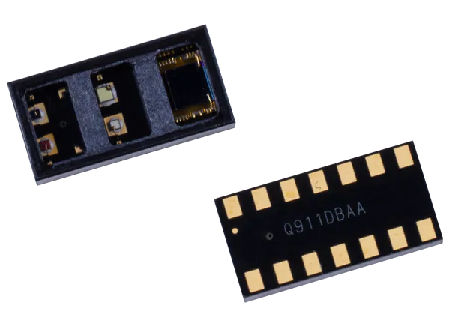
\includegraphics[width=0.6\linewidth]{ImageFiles/Hardware/MAX86916_Layout}
	\caption{MAX86916 magari mettere in evidenza led e foto diodo}
	\label{fig:xxxx}
\end{figure}

\paragraph{Sensore PPG} Il sensore PPG utilizzato è il MAX86916, prodotto da Maxim Integrated, descritto precedentemente come stato dell'arte.

\paragraph{LDO} \todo{Parliamo dei 3 LDO che abbiamo valutato? si parlerei di tutti e tre o almeno 2 mettendo in evidenza magari una tabella con le differenze}

\paragraph{Accelerometro}\todo{ut supra} L'accelerometro utilizzato è sempre \textbf{LIS2DH12} prodotto da STMicroelectronics.

\subsection{Microcontrollore: STM32F4DISCOVERY}\todo{farei una descrizione con alcune nozione sui componenti}
\todo{inserire immagine della board}